\documentclass[titlepage]{article}
\usepackage[spanish]{babel}
\usepackage[utf8]{inputenc}

\usepackage{natbib}

\usepackage{xcolor}
\definecolor{darkblue}{rgb}{0.1 , 0.1, 0.64}
% hyperrefs antes de geometry!
\usepackage[
hyperfootnotes=false,
urlcolor=blue,
colorlinks=true,
linkcolor=darkblue,
citecolor=red]{hyperref}


\usepackage{graphicx}
\usepackage{amsmath}
\title{ejemplo2}
\author{Patricio Whittingslow}
\date{October 2020}


\newcommand{\micomando}[0]{\textbf{Hola}: \textit{Chau}}

\newcommand{\hey}[2]{\textbf{#1}: \textit{#2} }

\begin{document}

\begin{titlepage}
\centering

\hey{Hey}{Chau}

{\sc Instituto Tecnologico de Buenos Aires \par}

\vspace{20mm}

{\Huge \bf Titulo de mi proyecto \par}
\vspace{30mm}
{ \large Patricio - {\bf 55423} \par}
\vspace{30mm}
{ \today \par }

\end{titlepage}

\tableofcontents

\section{Introduction}
\subsection{Subseccion }
\begin{figure}
    \centering
    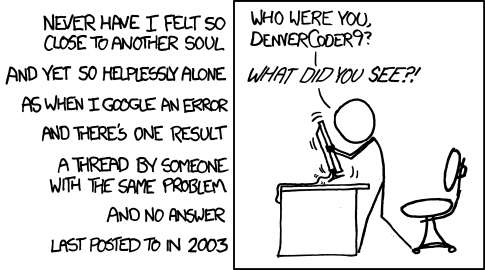
\includegraphics[width=0.4\textwidth]{fig/comic.png}
    \caption{Un comic que me gusta}
    \label{fig:primer_comic}
\end{figure}

\begin{figure}[h!]
    \centering
    
\includegraphics[width=0.4\textwidth]{fig2}
    \caption{Un comic que me gusta}
    \label{fig:primer_comic}
\end{figure}

Por favor dirijase a la figura \ref{fig:primer_comic}


\begin{table}[h!]
\centering
\begin{tabular}{rc|c|cc} % r c l
\multicolumn{2}{c}{Contenido Multicol}  & \textbf{dsdsa} & \textbf{} &  \\ \hline 
1             & 2               &                &           &  \\
3             & 3               & 3              &           &  \\
              &                 &                &           & 
\end{tabular}
\end{table}

\section{Matematica}
Mi matematica $d=1$, tambien $\frac{1}{2} = \pi$. 

\begin{equation} \label{eq:schrodinger}
    \Phi =  \frac{1}{2} \cdot \frac{\hbar + 2\pi }{\Gamma + c^{2} }
\end{equation}

\newcommand{\transform}[3]{ \ensuremath{\mathbf{T}^{#1}_{#2#3}}}

\begin{align}
    \Phi &=  \frac{1}{2} \cdot \frac{\hbar + 2\pi }{\Gamma + c^{2} } \\
    & = 0 \cdot 12312312312 \\
    & = \transform{A}{B}{G}
\end{align}

Segun vimos en la ecuacion \ref{eq:schrodinger}. \transform{A}{B}{G}. La luz es rápida \citep{serway}. La masa del pan es dura \cite{kawai}.

\bibliography{mibib}
\bibliographystyle{plainnat}

\end{document}
